\documentclass[conference]{IEEEtran}

%\usepackage[russian]{babel}
\usepackage[justification=centering]{caption}
\usepackage[backend=bibtex]{biblatex}
\usepackage{fontspec}
\usepackage{graphicx}
\usepackage{listings}
\usepackage{array}
\usepackage{xcolor}
\usepackage{graphicx}
\usepackage{tikz}
\usepackage{pgfplots}
%\usepackage{geometry}
\graphicspath{{./images/}}

\setmainfont{Spectral Light}%{Times New Roman}

\definecolor{codegreen}{rgb}{0,0.6,0}
\definecolor{codegray}{rgb}{0.5,0.5,0.5}
\definecolor{codepurple}{rgb}{0.58,0,0.82}
\definecolor{backcolour}{rgb}{0.95,0.95,0.92}

\lstdefinestyle{mystyle}{
    backgroundcolor=\color{white},   
    commentstyle=\color{codegreen},
    keywordstyle=\color{magenta},
    numberstyle=\color{codegray},
    stringstyle=\color{codepurple},
    basicstyle=\ttfamily\footnotesize,
    morekeywords={*,procedure, if, rol, cmpj, setmask, then, else, endif, cmpjn, is, not, and, return},            % if you want to add more keywords to the set
    breakatwhitespace=false,         
    breaklines=true,                 
    captionpos=b,                    
    keepspaces=true,                 
    numbers=left,                    
    numbersep=10pt,
    xleftmargin=7mm,
    xrightmargin=0mm,
    showspaces=false,                
    showstringspaces=false,
    showtabs=false,                  
    tabsize=4
}
\lstset{style=mystyle}
\lstset{linewidth=9cm}
\bibliography{monetec} 


\begin{document}
\title{
    Data Structures for Classification Table Search in the Network Processor without the Separate Associative Device
}
\maketitle
    \begin{abstract}
        This paper addresses the problem of the paket classification within a network processor (NP) architecture 
        without the Separate Associative device.
        By classification we mean the process of identifying a packet by its header.
        The classification stage requires the implementation of data structures to store the classification tables.
        In our work we consider NP without the associative memory,
        To classify the packets in such a NP, we propose to use search trees.
        On the basis of the implemetations of the considered architecture 
        data structures for the further evaluation have been chosen.
        An evaluation of the implemented data structures was carried out on a 
        simulation model of the network processor.
        Use of the adapted AVL tree showed that it allowed reducing 
        the number of network processor cycles for processing one packet and reducing the use of memory of the conveyor's computing blocks.
    \end{abstract}
    
    \begin{IEEEkeywords}
        Network processor, software-defined networks, packet classification, search trees.
    \end{IEEEkeywords}
    
    \section{Introduction}
        At present, the technology of the software-defined
        networks (SDN)~\cite{smel2012open} that require high-performance 
        switches~\cite{bifulco2018survey}. The main functional element of the high-perfomance SDN switches
        is a programmable network processor.
        The network processor (NP) is a System-On-Chip specialized for the network packet processing that performs the following functions:
        receiving a packet from a physical port, selecting a header,
        classification of the package by its header, decision on further 
        packet paths, send the packet to the physical port~\cite{chao2007high:1}.
        Programmable network processors are being actively developed.
        By programmable network processor we mean network processor, 
        which allows you to change the packet processing program and set of differentials 
        header fields, so you can quickly adjust to new protocols, 
        and use the switch in SDN networks~\cite{bezzubtsev2019ob-odnom183708319}.

		Based on the functions of the network processor, it is reasonable to consider the pipeline architecture. 
		It allows you to process each packet with a fixed delay. 
        The pipeline in the network processor consists of computing blocks. 
        This article will discuss the classification stage of packages.
        The classification is understood as the process of identification of a network packet 
        by its characteristics defined by the current protocol.
        The $-$ classification table is a set of rules, containing the characteristics, 
        by which the group of packets is identified,
        and the actions that the network processor performs on this group of packets. 
        Thus, to perform the classification, the network processor must include an associative device. 
		Associative memory is commonly used to implement this device.
        However, a single associative memory controller will be the bottleneck, 
        since it must be available for all stages of the pipeline.
        Accordingly, there is a need to make the architecture more complex, 
        for example, by adding several controllers of associative memory to it.
        To avoid complex organization of memory, it is possible to refuse using associative memory in architecture. 
        In this case one of the $-$ solutions is to combine the memory of commands 
        and data and place the memory on a network processor chip.
        Thus, the task of developing data structures for searching in classification 
        tables in the network processor without a dedicated associative device arises.

    \section{Network processor architecture}
        \label{section:problem}
        In considered network processor the conveyor architecture is used, each conveyor consists of 10 computing blocks. 
         
        Each computing block has access to the memory area where the microcode and data are located.
        There is a limit on the number of clock cycles that one packet can process on a processing block, 
        it corresponds to 25 clock cycles.
        This limit is due to the performance requirement of the network processor, 
        namely a fixed processing time per packet on the network processor.
        Also one computing unit has access to 2 megabytes of memory.
        Due to the micro architecture, there is no separate memory area where data is stored. 
        Therefore, the microcode contains all the data,needed to classify packages.


        \begin{figure}[h]
            \includegraphics[width=0.5\textwidth]{npu_all.png}
            %\includegraphics[]{npu_all.png}
            \caption{Network processor architecture}
        \end{figure}
        
        \subsection{Network processor asembler language}
            To describe network packet processing programs in the network processor architecture 
            under consideration, the assembler language is used. 
            The following classes of instructions are present in the language under consideration:
            \begin{itemize}
                \item Instructions for working with the register.
                \item Instructions for arithmetic operations.
                \item Instructions of bit operations.
                \item Instructions for conditional and unconditional transition to the label.
                \item Instructions for writing to the output port register.
            \end{itemize}.

    \section{Related work}
        Solutions to the problem are presented in the literature. 
        Due to the peculiarities of the network processor architecture, namely, the lack of 
        of the addressable memory, 
        that is required for non-timber data structures will be considered 
        only tree-like data structures. 
        
        The decisions under consideration will address the following aspects:
        {\bf asymptotic search complexity} $-$ makes it possible to evaluate the use of 
        network processor resources to search the data structure,
        {\bf data structure universality} $-$ used data structure
        should support the search for arbitrary bit strings not exceeding 128 bits in length,
        {\bf need to use Addressable Memory} $-$ to some under consideration 
        data structures need addressable memory to implement them, 
        corresponding to their asymptotic complexity,
        {\bf number of tops} that you need to visit to find
        in case of storing bit strings up to 48 bits long,
        {\bf need to change microarchitecture} of the conveyor's computing blocks 
        of a network processor,
        {\bf estimates the amount of memory} occupied by the data structure $-$ for 64000 occurrences of IPv4 prefixes.
        In the literature under consideration there are several main approaches to developing data structures, 
        to store the classification tables. Namely: using the principle of hash tables, using the principle of trees 
        and using the principle of balancing trees.

    \subsection{Method for calculating the memory size occupied by the data structure}
        For the data structure being implemented, the number of nodes for storing
        64000 bit strings $-$ $N$ is calculated, then the average number of instructions on 
        one tip of $-$$S$. Then the required memory size occupied by the data structure 
        will be calculated by the formula $M = instruction\_size * N * S$,
        where $instruction\_size = $128, due to the network processor architecture under consideration.

    \subsection{Hash table usage}
        This method uses addressable memory, so it was not considered in this paper. 
        As there is no possibility of addressable memory in the network processor architecture under consideration.
        One example of this approach is binary search by prefix lengths.
        The considered data structure is based on building special tables for prefixes of a certain length~\cite{mun2006binary}. 
        Let the maximum length of the prefix be {\ttfamily $W$}, then construct tables {\ttfamily $h_{1},\ldots,h_{w}$}. 
        Each of them stores length prefixes corresponding to this table number. 
        It is assumed that each such table has its own hash function, 
        which quickly allows you to find the prefix's entry in this table.
        In this way we can perform a binary search on the length of prefixes. 
        Within the framework of the network processor architecture in question, 
        Such tables can only be implemented using tree data structures~\cite{mun2006binary}. 

    \subsection{Tree usage}
        \label{section:bctrev}
            Most common~\cite{behdadfar2009scalar} data structure for searching by 
            the longest match is a binary one bit tree. 
            The tree is built according to the given prefixes so that each bit of the prefix has its own top in the tree. 
            The search is performed by lowering the bits of the element for which the search is performed. 
            The search ends when the empty vertex is reached, the search result is the last prefix~\cite{chao2007high:1}.
            The optimization of the one bit binary tree~\cite{ruiz2001survey} is a binary compressed tree. 
            To build this tree you must build a binary one bit tree, 
            then perform a compression procedure, namely all the vertices that have only one sheet, 
            are reduced, and the number of missed vertices is recorded at the next vertex. 
            Thus, the built tree has no vertices with one sheet. 
            Due to the described optimization, this tree takes less memory, 
            than a binary one bit tree. This is due to the lack of passing tops. 
            However, the number of search instructions spent only on 
            for prefixes that had single-leafed tops before them. For the worst case, when for a prefix there are all its shorter versions, the number of vertices, 
            that you need to visit to search, similar to the binary single-bit tree ~\cite{ruiz2001survey}. 

            Multi-bit compressed tree $-$ optimization of the binary compressed tree~\cite{berger2003ip}.
            A different tree structure is used when there may not be a maximum of two sheets in each vertex, 
            and {\ttfamily $2^h$}, where {\ttfamily $h$} $-$ is the maximum depth of the subtree of the top.
            When using this data structure within a general purpose processor architecture, 
            the number of operations to search is limited by the depth of the tree,
            which equals {\ttfamily $\frac{W}{K}$}, where {\ttfamily $W$} $-$ length of maximum prefix, 
            and {\ttfamily $K$} $-$ the number of levels in our tree.
            The implementation of this tree will be considered within the network processor architecture, 
            which uses a linear search in each node by child nodes~\cite{berger2003ip}.
                   
        \subsection{Balanced tree usage}
            \label{section:avlrev}
            Many different balancing trees have been considered in this category in the literature, such as: B-trees,
            red-black trees, AVL tree. All balancing trees use an algorithm for presenting prefixes.
            like scalar values.
            In this paper, the AVL tree was considered in detail as an example.
            Representing prefixes as scalar prefixes allows using a larger set of data structures~\cite{behdadfar2009scalar}. 
            As an example, let's consider the AVL tree, the main feature of which 
            is the rule of its construction: each vertex has a difference of 
            the depth of the left and right subtree is not greater than 1, which gives 
            asymptotic search complexity {\ttfamily $O(1+\log_2{N})$}, 
            where {\ttfamily $N$} $-$ the number of prefixes in our data structure. 
            It follows that the search time does not depend on the length of the data you are looking for,
            which means that using this data structure you can effectively search for IPv6~\cite{behdadfar2011coded} prefixes. 
            \\
    \subsection{Сравнение структур данных}
        Each reviewed data structure has its advantages and disadvantages, let us consider them:
        \begin{enumerate}
            \item \textbf{Binary single-bit tree} $-$ this structure is simple to implement but 
                takes up a lot of memory and the search requires 48 nodes.
            \item \textbf{Binary single-bit compressed tree} $-$ takes less memory than 
                a single-bit binary tree, but the search requires 48 nodes. 
                Accordingly, using this tree is preferable to a single-bit binary tree.
            \item \textbf{Multi-bit compressed tree} $-$ occupies a lot of memory, but search requires a much smaller number of vertices. 
                Due to implementation problems within the framework of the architecture in question, this data structure cannot be implemented.
            \item \textbf{Binary prefix length search} $-$ occupies a lot of memory, and can only be used to find the longest prefix.
                Also, due to implementation problems on the architecture in question, this structure is not suitable for solving the problem.
            \item \textbf{AVL tree} $-$ occupies the least amount of memory, and the search requires a small number of nodes,
                which depends on the number of occurrences in the data structure rather than the specific prefix.
        \end{enumerate}

        Thus, based on the review, it is appropriate to select two data structures for further implementation: 
        AVL tree with an algorithm for representing prefixes as scalar values and a binary compressed tree. 
        A binary single-bit tree has also been selected as a reference.

\section{Proposed data structures}
    \label{section:trees}
        The description of the algorithms used the data structure \emph{Node}, which contains the following fields:
        \begin{itemize}
            \item \emph{Node.left} $-$ link to the left son of the top.
            \item \emph{Node.right} $-$ link to the right son of the vertex.
            \item \emph{Node.rule} $-$ action corresponding to the prefix of the vertex.
            \item \emph{Node.prefix} $-$ prefix of the current vertex.
            \item \emph{Node.bit} $-$ significant bit in the current vertex.
        \end{itemize}
        And the structure \emph{prefix}, which contains the following fields:
        \begin{itemize}
            \item \emph{prefix.bit\_string} $-$ bit string setting the prefix.
            \item \emph{prefix.length} $-$ prefix length. When looking for an exact match, 
                the length of the prefix is the length of the bit string.
        \end{itemize}.
    
    \subsection{Binary one bit tree}
        \label{section:binone}
            Let's consider an algorithm for building a binary one bit tree,
            which is the base for a binary compressed tree.
            To add nodes to the data structure let's define the procedure \emph{Add} (Listing~\ref{lst1}). 
            \\
            {\bf Input:} current node \emph{Node}, added prefix \emph{prefix}, 
            rule for the current prefix \emph{rule}, and current bit \emph{bit}. 
            \\
            {\bf Output:} updated current top, namely the structure object \emph{Node}.
\\
\begin{lstlisting}[caption=Procedure for adding a vertex to a binary one bit tree., label=lst1]
procedure Add(Node, prefix, rule, bit)
    if Node is empty then
        Node = new Node()
        Node.bit = bit
    endif
    if prefix.length == bit then
        Node.prefix = prefix
        Node.rule = rule
        Node.bit = bit
        return Node
    endif
    if prefix.bit_string[bit] == 1 then
        Node.left = Add(Node.left, prefix, rule, bit + 1)
    else
        Node.right = Add(Node.right, prefix, rule, bit + 1)
    endif
    return Node
\end{lstlisting}
\vspace{1em}
            Therefore, to build a binary single-bit tree, all rules from the classification table 
            must be added sequentially, using the procedure \emph{Add}.

        \subsection{Binary compressed tree}
            Let's consider the algorithm of building a compressed binary tree. 
            To simplify the software implementation, first a binary one bit tree was built,
            The procedure of building which is described in point~\ref{section:binone}. 
            To obtain a compressed binary tree from the built binary one bit tree,
            all the tops that have only one son and no prefix should be removed.
            \subsubsection{Procedure to remove insignificant vertices}
                Consider the procedure for removing \emph{Remove} insignificant vertices 
                from a binary one bit tree to obtain a binary compressed tree. 
                \\
                {\bf Input:} current vertex \emph{Node}.
                \\
                {\bf Output:} updated current top \emph{Node}.
                The algorithm for removing unimportant vertices can be represented 
                as a procedure pseudo code \emph{Remove} (Listing~\ref{lst2}).
\\
\begin{center} 
\begin{lstlisting}[caption=The procedure for removing insignificant vertexes., label=lst2]
procedure Remove(Node):
    if Node.prefix is empty then
        if Node.left is empty and Node.right is not empty then
            return Node.right
        endif
        if Node.left is not empty and Node.right is empty then
            return Node.left
        endif
    else
        return Node
    endif
\end{lstlisting}
\end{center}
\vspace{1em}
            This algorithm allows you to build a compressed binary tree based on a binary one bit tree 
            by removing insignificant vertices from a single-bit binary tree. \\
            For this tree it was necessary to develop a procedure describing the vertex 
            of the considered data structure. This procedure should make it possible to execute
            to search the built data structure.
            Let's consider the procedure describing the vertex of the binary compressed tree 
            within the limits of the considered architecture of the network processor:
\\
\begin{lstlisting}[caption=Procedure for describing the tip of a compressed binary tree.]
setmask (1 << port)
cmpj lable, prefix.bit_string, prefix.length
\end{lstlisting}
\vspace{1em}
            In this procedure:
            \emph{setmask 1 <\,< port} $-$ is an optional instruction 
            and is only present when the current vertex has a prefix.
            \emph{cmpj label, prefix.bit\_string, prefix.length} $-$ comparison in the current vertex, 
            then you go to \emph{label}, otherwise the program just keeps running.
            The \emph{label} $-$ tag can be in front of the left son if it is otherwise labeled \emph{finish},
            which terminates the program and thus stops searching the data structure.
        \subsection{AVL tree}
            \subsubsection{Algorithm for representing prefixes as scalar values}
                This algorithm is necessary to save and search for prefixes in the AVL tree, 
                because initially only scalar values can be stored in the tree tops.
                The algorithm allows comparing prefixes with each other~\cite{behdadfar2011coded}, namely:
                \begin{itemize}
                    \item If the lengths of the two prefixes match, they are compared as two scalar values.
                    \item If the length of the $q$ prefix is smaller than the length of the $p$ prefix, 
                        the first $len(q) - 1$ bits of both prefixes are compared as scalar values.
                \end{itemize}
                This algorithm can be described by the procedure \emph{PrefixCompare} (Listing~\ref{lst3}). 
                \\
                {\bf Input:} prefix \emph{prefix1} and prefix \emph{prefix2}. 
                \\
                {\bf Output:} \emph{True}, if the first prefix is greater than the second, otherwise \emph{False}.
\\
\begin{lstlisting}[caption=Procedure for comparing prefixes as scalar values., label=lst3]
procedure PrefixCompare(prefix1, prefix2):
    if prefix1.length == prefix2.length then
        return Int(prefix1.bit_string) > Int(prefix2.bit_string)
    else
        minimal_length = Min(prefix1.length, prefix2.length) - 1
        return Int(prefix1.bit_string[0:minimal_length]) > Int(prefix2.bit_string[0:minimal_length])
    endif
\end{lstlisting}
            \subsubsection{Tree building algorithm}
                Let's consider the algorithm of building the AVL tree, 
                namely adding new vertices to it. This algorithm can be 
                described by the procedure \emph{Add} (Listing~\ref{lst4}).
                To build the AVL tree we use the structure \emph{Node}, 
                which is identical to the structure described at \ref{section:binone}.
                \\
                {\bf Input:}
                \begin{itemize}
                    \item \emph{Node} $-$ object of the AVL tree top structure.
                    \item \emph{prefix} $-$ current prefix.
                    \item \emph{rule} $-$ rule for the current prefix.
                \end{itemize}
                {\bf Output:} updated current top \emph{Node}.
                \\
                Also \emph{Add} uses the procedure \emph{BalanceNode}, 
                which performs the AVL balancing operation on the tree.
                \\
\begin{lstlisting}[caption=Procedure for adding the vertex to the AVL tree., label=lst4]
procedure Add(Node, prefix, rule):
    if Node.prefix is empty then
        return new Node(prefix, rule, depth=1)
    endif
    
    if prefixCompare(prefix, Node.prefix) then
        Node.right = Add(Node.right, prefix, rule)
    else:
        Node.left = Add(Node.left, prefix, rule)
    endif
    
    return BalanceNode(Node)
\end{lstlisting}
\vspace{1em}
This procedure allows you to build an AVL tree by successively adding rules from the table.
    \section{Experimental study}
        \subsection{Network Processor Simulation Model}
            A $-$ network processor simulation model is a software tool written 
            in the python programming language that allows you to simulate network processor operation, 
            Namely, receive packets on any of the 24 ports, process the packet, 
            receiving information about any stage of processing, and send the packet to the output ports.
            A simulated network processor model allows you to estimate 
            the number of clock cycles spent to process the packet, 
            as well as the amount of memory spent on the data structure.
        
            Packets are sent to the network processor ports using $pcap$ files, 
            which can describe how packets are received on each port at certain points in time.
            In this paper, without limiting the commonality, only one port of the 
            network processor simulation model will be considered. Since for each input port
            the port uses a suitable conveyor. In the conveyor of the network processor 
            simulation model one computing unit is implemented, it is enough to perform 
            experimental study, as the network processor pipeline has a static schedule.

            The source program for packet processing is accepted as code 
            written in assembler language which is used in the network processor architecture under consideration.
            The simulation model converts the program by expanding 
            the directives $\#include$ and $\#define$, and starts to simulate the network processor for this program.
 
        \subsection{Software Implementation Description}
            For further experimental research it is necessary 
            to develop a software implementation in python language. 
            The software implementation should include the following modules:
        
            \begin{itemize}
                \item Module to download classification tables from a file.
                \item AVL-tree building module.
                \item Binary compressed tree building module.
                \item Module of building a single-bit binary tree.
                \item The module of building the constructed tree in assembler language.
            \end{itemize}.
            
            The scheme of interaction of modules is shown in Figure~\ref{fig:mesh5}.

        \begin{figure}[ht]
            \centering
            \includegraphics[width=0.5\textwidth]{program_scheme.jpg}
            \caption{The scheme if software implementation}\label{fig:mesh5}
        \end{figure}

            \subsubsection{Classification tables load module}
            \label{section:tablemod}
                This module reads files of classification tables and converts them to a dictionary where the key is a bit string,
                and the value is the switch port number. These dictionaries are sent to data structure modules.
                The module allows using existing classification tables for experimental research.
                An example of classification input tables is presented in listing~\ref{lst6}.
                \\
\begin{lstlisting}[caption=Example of classification table., label=lst6]
{IPv4}
192.168.31.0 24 1
192.168.43.0 24 2
\end{lstlisting}
            \subsubsection{Modules for building data structures}.
                These modules implement the construction of the described trees, namely, 
                a binary compressed tree, a binary one bit tree and the AVL tree.
                The modules take the read from the file and the converted classification tables as input.
                Then each rule is sequentially added to the data structure, 
                the algorithm of addition is described in chapter~\ref{section:trees}, 
                for each of the of the data structures under consideration.
                After building the data structure is transferred to the module 
                of tree conversion to the assembler language used in the network processor as a root vertex.

            \subsubsection{Module of building the transformation of the built tree into the assembler language}.
                For each tree the conversion module builds a certain assembler code, 
                which is described in detail in chapter~\ref{section:trees}.
                The transformation takes place recursively through the tree structure, 
                the nodes are sequentially written into an array, and then
                a separate assembler code is generated for each vertex.
                The generated assembler code is written to the specified file. 
                Then the file is used for experimental investigation on a network processor simulation model.
                An example of converting a compressed binary tree 
                from point~\ref{section:bctrev} is presented in listing~\ref{lst7}.
\\
\begin{lstlisting}[caption=Example of a compressed binary tree in assembly language., label=lst7]
cmpj l_1, 1, 1
setmask (1 << 3)
cmpjn finish, 1, 2
setmask (1 << 1)
j finish

l_1:
cmpj l_2, 11, 2
cmpjn finish, 101, 3
setmask (1 << 5)
cmpjn finish, 1011, 4
setmask (1 << 6)
j finish

l_2:
setmask (1 << 4)
cmpjn finish, 1100, 4
setmask (1 << 2)
j finish

finish:
\end{lstlisting}
        \subsection{Method of experimental research}
            For the experimental study were found tables of switching prefixes of different lengths. 
            The experimental study will be conducted for different size classification tables, 
            namely: 1000, 8000, 16000, 32000, 64000 bit rows. Bit rows of different lengths will be used, namely:
            32, 48 bits. For each data structure, studies will be carried out with traffic 
            covering the loaded table into a simulated network processor model.
            Research will also be performed to find the longest prefix and the exact match.
            To conduct an experimental study, you will need to perform the following steps:
            \begin{enumerate}
                \item Prepare the input data for the software implementation, 
                    i.e.\ bring the classification tables to the type described in point~\ref{section:tablemod}.
                \item For each of the classification tables under consideration construct 
                    developed data structures and transform them into assembler code.
                \item Simulate for each data structure on a network processor simulation model.
                \item Fix the received data during the simulation, namely, 
                    the amount of the consumed memory of the network processor conveyor 
                    and the average number of instructions to classify the package.
            \end{enumerate}

            For a compressed binary tree, a significant reduction in memory capacity 
            and a reduction in the average number of cycles per batch is expected
            compared to a binary single-bit tree.
            For the AVL tree, a decrease in the average number of cycles per packet 
            is expected compared to a binary compressed tree and a decrease 
            in the average number of cycles per packet compared to a binary compressed tree
            not a strong reduction in the amount of memory used to store the data structure.
    \section{Evaluation}
        This section presents the results of an evaluation of developed data structures 
        for size classification tables from 1000 to 64000, and signs of different lengths.
        \subsection{Binary one bit tree}
            Let's consider the graph of dependence of the average number of instructions spent 
            on search by data structure for the package on the number of rules in the classification table (Fig.~\ref{graph:btinst}).
            
            \begin{figure}[!htbp]
                \centering
            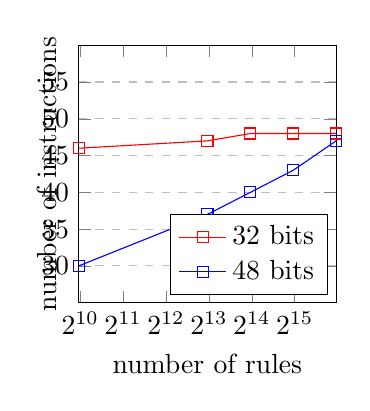
\begin{tikzpicture}
            \begin{axis}[
                width=0.4\textwidth,
                height=0.4\textwidth,
                ylabel={number of instructions},
                xlabel={number of rules},
                y label style={at={(-0.05, 0.5)}},
                ymin=25, ymax=60,
                xmin=1000, xmax=64000,
                xmode=log,
                log basis x={2},
                xtick={0, 128, 256, 512, 1024, 2048, 4096, 8192, 16384, 32768},
                ytick={30, 35, 40, 45, 50, 55},
                legend pos=south east,
                ymajorgrids=true,
                grid style=dashed,
                cycle list name=color list] 
                \addplot+[mark=square] coordinates{(1000, 46)(8000, 47)(16000, 48)(32000, 48)(64000, 48)};
                \addplot+[mark=square] coordinates{(1000, 30)(8000, 37)(16000, 40)(32000, 43)(64000, 47)};
                \legend{32 bits, 48 bits}
            \end{axis}
            \end{tikzpicture}
                \captionsetup{justification=centering}
                \caption{Dependence number of instructions from number of rules.}
                \label{graph:btinst}
            \end{figure}
            As can be seen from the chart below, the average number of spent instructions
            practically does not change depending on the size of the classification table.
            On average, the number of instructions per package is 48 for 32-bit bit rows, and on average, 41 for 48-bit rows.
            Now let's look at the graph of dependence of the spent memory size 
            on the number of rules in the classification table (Fig.~\ref{graph:btmem}).
            \begin{figure}[!htbp]
                \centering
            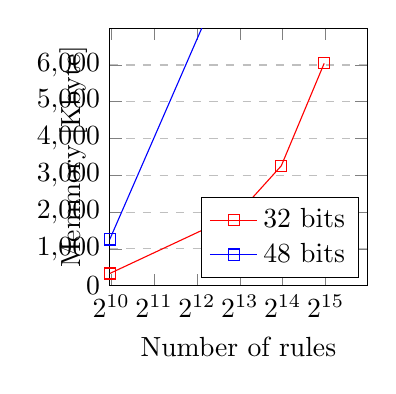
\begin{tikzpicture}
            \begin{axis}[
                width=0.4\textwidth,
                height=0.4\textwidth,
                ylabel={Memmory [Kbyte]},
                xlabel={Number of rules},
                y label style={at={(-0.05, 0.5)}},
                ymin=0, ymax=7000,
                xmin=1000, xmax=64000,
                xmode=log,
                log basis x={2},
                xtick={0, 128, 256, 512, 1024, 2048, 4096, 8192, 16384, 32768},
                ytick={0, 1000, 2000, 3000, 4000, 5000, 6000},
                legend pos=south east,
                ymajorgrids=true,
                grid style=dashed,
                cycle list name=color list] 
                \addplot+[mark=square] coordinates{(1000, 328.64)(8000, 1966.62)(16000, 3258.27)(32000, 6045.09)};
                \addplot+[mark=square] coordinates{(1000, 1255.16)(8000, 9287.18)};
                \legend{32 bits, 48 bits}
     
            \end{axis}
            \end{tikzpicture}
                \captionsetup{justification=centering}
                \caption{Dependence of memory from number of rules.}
                \label{graph:btmem}
            \end{figure}
            From the presented graph, you can see that a binary one bit tree takes up several 
            times more memory than the limitations presented in chapter~\ref{section:problem}.
            This does not allow using this data structure in the network processor architecture under consideration.
        \subsection{Binary compressed tree}
            Let's consider the graph of dependence of the average number of instructions 
            spent on search by data structure for the package on the number of rules 
            in the classification table (Fig.~\ref{graph:compinst}).
            \begin{figure}[h!]
                \centering
            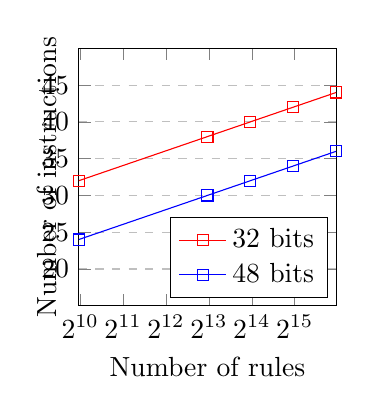
\begin{tikzpicture}
            \begin{axis}[
                width=0.4\textwidth,
                height=0.4\textwidth,
                ylabel={Number of instructions},
                xlabel={Number of rules},
                y label style={at={(-0.05, 0.5)}},
                ymin=15, ymax=50,
                xmin=1000, xmax=64000,
                xmode=log,
                log basis x={2},
                xtick={0, 128, 256, 512, 1024, 2048, 4096, 8192, 16384, 32768},
                ytick={20, 25, 30, 35, 40, 45},
                legend pos=south east,
                ymajorgrids=true,
                grid style=dashed,
                cycle list name=color list] 
                \addplot+[mark=square] coordinates{(1000, 32)(8000, 38)(16000, 40)(32000, 42)(64000, 44)};
                \addplot+[mark=square] coordinates{(1000, 24)(8000, 30)(16000, 32)(32000, 34)(64000, 36)};
                \legend{32 bits, 48 bits}
     
            \end{axis}
            \end{tikzpicture}
                \captionsetup{justification=centering}
                \caption{Dependence number of instructions from number of rules.}
                \label{graph:compinst}
            \end{figure}
            As can be seen from the chart below, the average number of spent instructions 
            practically does not change depending on the size of the classification table.
            On average, the number of instructions per package is 39 for 32-bit bit rows, 
            and on average 31 for 48-bit rows.
            Now let's look at the graph of dependence of the spent memory size on the number 
            of rules in the classification table (Fig.~\ref{graph:compmem}).
            \begin{figure}[!htbp]
                \centering
            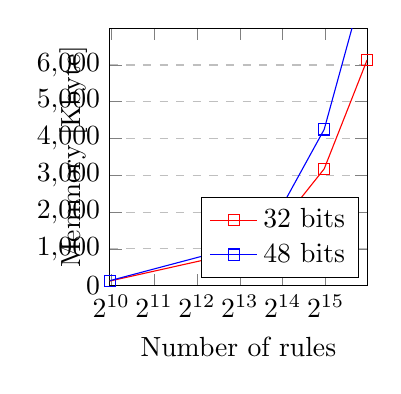
\begin{tikzpicture}
            \begin{axis}[
                width=0.4\textwidth,
                height=0.4\textwidth,
                ylabel={Memmory [Kbyte]},
                xlabel={Number of rules},
                y label style={at={(-0.05, 0.5)}},
                ymin=0, ymax=7000,
                xmin=1000, xmax=64000,
                xmode=log,
                log basis x={2},
                xtick={0, 128, 256, 512, 1024, 2048, 4096, 8192, 16384, 32768},
                ytick={0, 1000, 2000, 3000, 4000, 5000, 6000},
                legend pos=south east,
                ymajorgrids=true,
                grid style=dashed,
                cycle list name=color list] 
                \addplot+[mark=square] coordinates{(1000, 123.58)(8000, 904.71)(16000, 1709.80)(32000, 3174.94)(64000, 6135.29)};
                \addplot+[mark=square] coordinates{(1000, 133.13)(8000, 1060.78)(16000, 2124.25)(32000, 4247.97)(64000, 8497.06)};
                \legend{32 bits, 48 bits}
     
            \end{axis}
            \end{tikzpicture}
                \captionsetup{justification=centering}
                \caption{Dependence of memory from number of rules.}
                \label{graph:compmem}
            \end{figure}
            You can see from the presented graph that the compressed binary 
            tree takes more memory than in the limitations presented in chapter~\ref{section:problem}, 
            only at 32000 of the rules in the classification tables.

        \subsection{AVL tree}
            Let's consider the graph of dependence of the average number of instructions 
            spent on search by data structure for the package on the number of rules 
            in the classification table (Fig.~\ref{graph:avlinst}).
            \begin{figure}[ht]
                \centering
            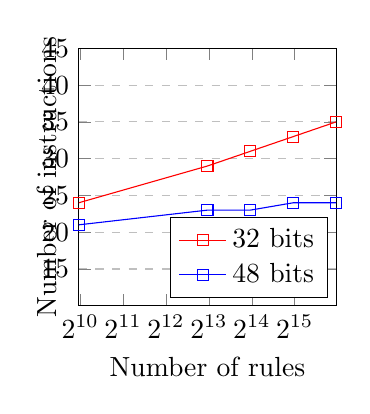
\begin{tikzpicture}
            \begin{axis}[
                width=0.4\textwidth,
                height=0.4\textwidth,
                ylabel={Number of instructions},
                xlabel={Number of rules},
                y label style={at={(-0.05, 0.5)}},
                ymin=10, ymax=45,
                xmin=1000, xmax=64000,
                xmode=log,
                log basis x={2},
                xtick={0, 128, 256, 512, 1024, 2048, 4096, 8192, 16384, 32768},
                ytick={15, 20, 25, 30, 35, 40, 45},
                legend pos=south east,
                ymajorgrids=true,
                grid style=dashed,
                cycle list name=color list] 
                \addplot+[mark=square] coordinates{(1000, 24)(8000, 29)(16000, 31)(32000, 33)(64000, 35)};
                \addplot+[mark=square] coordinates{(1000, 21)(8000, 23)(16000, 23)(32000, 24)(64000, 24)};
                \legend{32 bits, 48 bits}
     
            \end{axis}
            \end{tikzpicture}
                \captionsetup{justification=centering}
                \caption{Dependence number of instructions from number of rules.}
                \label{graph:avlinst}
            \end{figure}
            \\
            As can be seen from the graph below, the average number of spent instructions 
            practically does not change depending on the size of the classification table. 
            The average number of instructions per package is 30 instructions for 32-bit bit rows, 
            and on average 23 instructions for 48-bit bit rows.
            Now let's look at the graph of dependence of the spent memory size on 
            the number of rules in the classification table (Fig.~\ref{graph:avlmem}).
            \\
            \begin{figure}[ht]
                \centering
            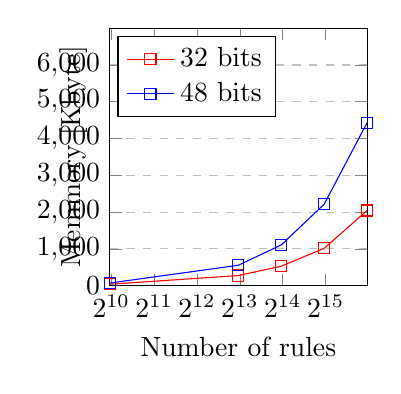
\begin{tikzpicture}
            \begin{axis}[
                width=0.4\textwidth,
                height=0.4\textwidth,
                ylabel={Memmory [Kbyte]},
                xlabel={Number of rules},
                y label style={at={(-0.05, 0.5)}},
                ymin=0, ymax=7000,
                xmin=1000, xmax=64000,
                xmode=log,
                log basis x={2},
                xtick={0, 128, 256, 512, 1024, 2048, 4096, 8192, 16384, 32768},
                ytick={0, 1000, 2000, 3000, 4000, 5000, 6000},
                legend pos=north west,
                ymajorgrids=true,
                grid style=dashed,
                cycle list name=color list] 
                \addplot+[mark=square] coordinates{(1000, 36.75)(8000, 273.48)(16000, 528.73)(32000, 1013.71)(64000, 2042.61)};
                \addplot+[mark=square] coordinates{(1000, 69.32)(8000, 553.59)(16000, 1107.23)(32000, 2213.89)(64000, 4429.01)};
                \legend{32 bits, 48 bits}
     
            \end{axis}
            \end{tikzpicture}
                \captionsetup{justification=centering}
                \caption{Dependence of memory from number of rules.}
                \label{graph:avlmem}
            \end{figure}
            \\
            You can see from the presented graph that the AVL tree fits 
            into the limitations presented in chapter~\ref{section:problem}, except for the case,
            when there are 64,000 rules in the classification table with 48 bit lengths.
        \subsection{comparison of data structures}
            This item presents a comparison of implemented data structures. 
            Let's consider the comparison charts of all implemented data structures.
            The first graph (Fig.~\ref{graph:allinst}) shows the comparison of 
            implemented data structures by the average number of instructions per one package. 
            You can see that the AVL tree shows the best result of all the implemented data structures.
            \\
            \begin{figure}[ht]
                \centering
            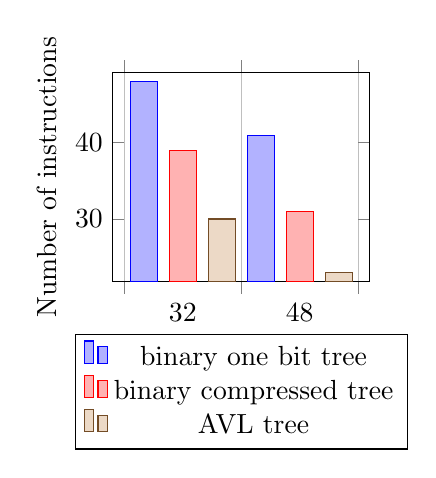
\begin{tikzpicture}
            \begin{axis}[
	            x tick label style={
		        /pgf/number format/1000 sep=},
                height=0.35\textwidth,
                width=0.4\textwidth,
	            ylabel=Number of instructions,
                xlabel=Bits,
	            enlargelimits=0.05,
	            legend style={at={(0.5,-0.25)},
	            anchor=north,legend columns=1},
	            ybar interval=0.7,
            ]
                \addplot coordinates {(32, 48)(48, 41)(64, 23)};
                \addplot coordinates {(32, 39)(48, 31)(64, 23)};
                \addplot coordinates {(32, 30)(48, 23)(64, 23)};
                \legend{binary one bit tree, binary compressed tree, AVL tree}
            \end{axis}
            \end{tikzpicture}
                \captionsetup{justification=centering}
                \caption{Compare number of instructions from bits in prefix}
                \label{graph:allinst}
            \end{figure}
            \\
            The following chart shows the comparison of implemented data structures 
            by the maximum memory size occupied by the data structure (Fig.~\ref{graph:allmem}). 
            You can see that only the AVL tree satisfies
            the restriction is presented in point~\ref{section:problem}, 
            and takes up much less memory than other data structures.
            \\
            \begin{figure}[ht]
                \centering
            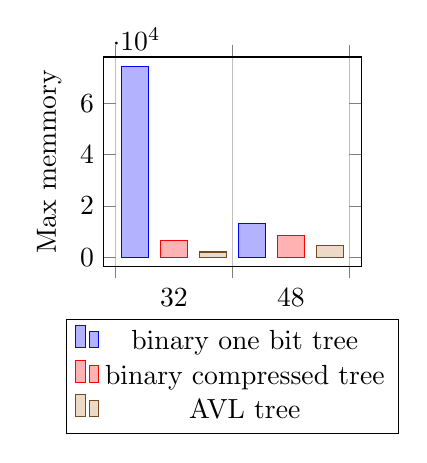
\begin{tikzpicture}
            \begin{axis}[
	            x tick label style={
		        /pgf/number format/1000 sep=},
                height=0.35\textwidth,
                width=0.4\textwidth,
	            ylabel=Max memmory,
                xlabel=bits,
	            enlargelimits=0.05,
	            legend style={at={(0.5,-0.25)},
	            anchor=north,legend columns=1},
	            ybar interval=0.7,
            ]
                \addplot coordinates {(32, 74231)(48, 13082)(64, 23)};
                \addplot coordinates {(32, 6532)(48, 8497)(64, 23)};
                \addplot coordinates {(32, 2042.61)(48, 4429.01)(64, 23)};
                \legend{binary one bit tree, binary compressed tree, AVL tree}
            \end{axis}
            \end{tikzpicture}
                \captionsetup{justification=centering}
                \caption{Comparison of the maximum amount of memory occupied by data structures.}
                \label{graph:allmem}
            \end{figure}
            \\
    \section{Conclusion}
        In this paper the problem of classifying packets in the considered architecture of the network processor was considered.
        Data structures have been developed to classify packets in the architecture in question.
        As part of this work, the following results were achieved:
        \begin{itemize}
            \item A review of existing solutions was carried out to select data structures 
                for further adaptation and implementation within the network processor architecture under consideration.
                Based on this review, the AVL tree and the binary compressed tree were selected.
            \item The selected data structures were adapted to the network processor architecture under consideration.
            \item The adapted data structures were implemented using the $python$ programming language.
            \item Additional software tools have also been developed for the experimental study.
            \item An experimental study was carried out, as a result of which characteristics 
                of the investigated data structures were obtained.
                For the AVL tree of $-$ tree the maximum memory size occupied 
                by the data structure doesn't exceed 2 MB and the average amount of
                instructions for classifying one package is 30 and 23 for 32-bit and 48-bit bit strings respectively.
                For the $-$ Binary Compressed Tree, the maximum amount of memory occupied 
                by the data structure does not exceed 8.5 MB, and the average number of
                instructions for classifying one package is 39 and 31 for 32-bit and 48-bit bit strings respectively.
            \item It was concluded from the data obtained during the experimental study that only the AVL tree satisfies the limitations,
                set out in this paper.
        \end{itemize}

        As a direction for further research, we can indicate a study of the possibility of further optimization of implemented data structures,
        to reduce the amount of memory occupied by data structures, as well as to consider changes in the network processor architecture
        and structures that require changes to the architecture in question.

\printbibliography{}
\end{document}
